% %%%%%%%%%%%%%%%%%%%%%%%%%%%%%%%%%%%%%%%%%%%%%%%%%%%%%%%%%%%%%%%%%%%%%%
% Dummy Chapter:
% %%%%%%%%%%%%%%%%%%%%%%%%%%%%%%%%%%%%%%%%%%%%%%%%%%%%%%%%%%%%%%%%%%%%%%

% %%%%%%%%%%%%%%%%%%%%%%%%%%%%%%%%%%%%%%%%%%%%%%%%%%%%%%%%%%%%%%%%%%%%%%
% The Introduction:
% %%%%%%%%%%%%%%%%%%%%%%%%%%%%%%%%%%%%%%%%%%%%%%%%%%%%%%%%%%%%%%%%%%%%%%
\fancychapter{Architecture}
\label{cap:architecture}

This chapter gives an overview of the state of the art of Indoor positining solutions. The \acf{BLE}'s architecture and functionality is analyzed in section \ref{sec:ble}, while section \ref{sec:indoortech} overviews the other existing technologies. The most common techniques utilized for position computation along side examples which make use of them are explained in section \ref{sec:techniques}. Finnally on section \ref{sec:related} analyzes the most projects that had the most relevance in the field and the existing work related to \ac{BLE}.

\section{Generic Architecture}
\label{sec:generic}



SystemRequisites
		Funcionais	
			- Capaz de comunicar com servidores (net)
			- ter required technologies????
			- ser capaz de funcionar diferentes implementações do mesmo sistema ( same shit different building)
			- beacon component must contain/indicate server where location is obtained

		Ambientais
		

		Energia
			- gastar menos que o gps, i guess


		Interoperacionais
			- Capacidade de funcionar com diferentes tipos de inputs, dependendo do que o utilizador decidir
			- data uniform






The solution presented in this paper was made with the objective of creating a generic indoor location system capable of being implemented using any existant indoor system created. The generic system's architecture is presented in figure ~\ref{fig:generic} and it's divided in 4 parts: beacon, location server, map server and smartphone application. 

\begin{figure}
	\centering
		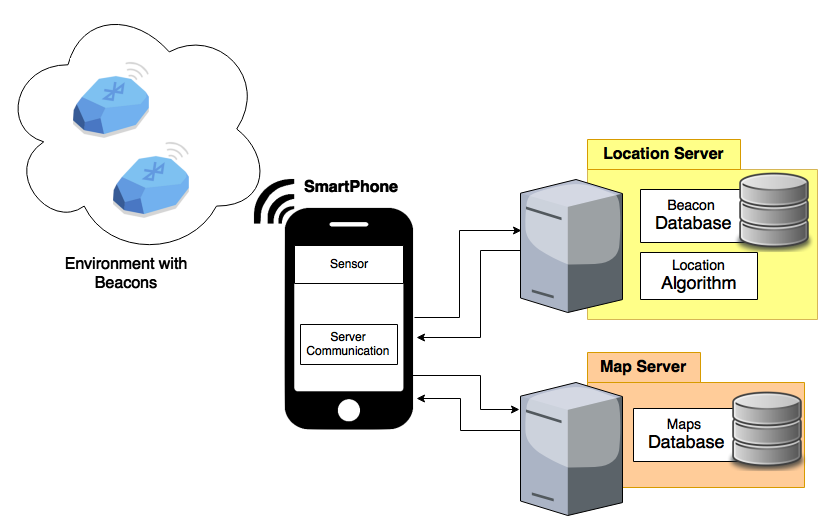
\includegraphics[width=1\linewidth]{3.Chapter/generic.png}
	\caption[Generic System's Architecture]{Generic System's Architecture}
	\label{fig:generic}
\end{figure}

The beacon represents any form of hardware responsible for providing fixed reference points which are fundamental in calculating a user's position. A beacon needs to be be composed of two structural blocks: The Unique ID, which stores any information crucial to identifying a beacon, and the Hardware specific software component, which contains all the necessary software to accomplish communication with a certain technology. 

The location server is divided in three: the Communication block, which is responsible for creating, managing and terminating a connection with the mobile application; the location algorithm, architectural block responsible for applying a certain location algorithm to the data received from the application in conjuntion with the server's device information in order to obtain a concrete location; and the beacon manager which functions as a database where all the beacon associated with the server are stored.

The map server represents the architectural block responsible for providing the maps associated to the location of user obtained through the location service on the application. As such it requires a communication block which needs to be capable of communication with the map service of the application and takes care of creating, managing and terminating connections, and a map manager which stores the existing maps that are to be transfered to the application.

The smartphone application is divided into three functional blocks: core application, location service and map service. The core application contains the core functionality of the application and is in charge of communicating with the existing services. Communication with the location service allows for requesting the user's location which is then forwarded to the map service, in order to obtain the associated map. The location service is composed by four blocks: the API component through which it communicates with the core of the application; the tag reader which is the functional block responsible for reading a certain type of tags (beacons) and as such its structure will depend on the type of beacon utilized by the service; the tag decoder, functional block responsible of utilizing the information obtained through the tag reader and process it in order to be forwarded to communication block; the communication block which takes care of the creating, managing and terminating connections with a location server.

It might be relevant to analyze some types of indoor location system that could diverge from this architecture, such as camera or Quick Response (QR) code-based systems. These systems would still follow the proposed architecture except for the beacon component which would not be existant and the location service's tag reader block wouldn't need any sort of communication since it would be responsible of utilizing the camera to capture either a fotograph or reading a QR core.


\begin{figure}
	\centering
		\includegraphics[width=0.75\linewidth]{3.Chapter/altgeneric.png}
	\caption[Adjustments to the application required for multiple indoor location systems]{Adjustments to the application required for multiple indoor location systems}
	\label{fig:altgeneric}
\end{figure}

Although figure \ref{fig:generic} is representative of a system utilizing a single type of technology, the presented solution is scalable, allowing for insertion of additional indoor location systems onto a single architecture. The changes required for implementing such a scenario would be to add one extra layer of complexity on the android application as present on figure \ref{fig:altgeneric}. In this new architecture, the application's core would only communicate with the location manager and the latter would now be responsible of managing through all of the location services and request execution of whichever service would be more suited or available. The location manager would also be required to manage through the existant map services, which may or may not be in same number as the existant location services, and make sure that the data obtained from a certain location service is forwarded to the correct map service which must capable of processing it.






\cleardoublepage
